% !TeX root = 数字电路.tex
% ============================================================
%  第二章 布尔代数
%  来源：笔记《布尔代数.md》与 Figure/ 中的逻辑符号图
% ============================================================
\chapter{布尔代数}
\label{chap:布尔代数}

数字电路的基础为逻辑代数，由英国数学家 George Boole 在 1847 年提出，逻辑代数也称布尔代数。

\section{基本逻辑运算}
\label{sec:基本逻辑运算}

在逻辑代数中，变量常用字母 $A,B,C,\cdots,Y,Z$、$a,b,c,\cdots,x,y,z$ 等表示，变量的取值只能是“0”或“1”。

逻辑代数中只有三种基本逻辑运算，即“与”、“或”、“非”。

\subsection{与逻辑运算}
\label{sec:与逻辑运算}

\begin{definition}[与逻辑运算]
	只有决定一事件的\textbf{全部条件}都具备时，这件事才成立；如果有一个或一个以上条件不具备，则这件事就不成立。这样的因果关系称为“与”逻辑关系，其函数式为 $F=A\cdot B=AB$。

	与门逻辑功能概括：\textcolor{red}{有“0”出“0”，全“1”出“1”}。
\end{definition}

与门逻辑符号如下：

\begin{figure}[H]
	\centering
	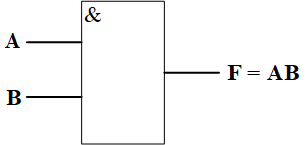
\includegraphics[width=0.3\linewidth]{Figure/与逻辑电路.png}
	\caption{与门逻辑符号}
	\label{fig:与门逻辑符号}
\end{figure}

与逻辑真值表如下：

\begin{table}[H]
\centering
\caption{与逻辑真值表}
\label{tab:真值表:与}
\begin{tabular}{cc|c}
	\toprule
	$A$ & $B$ & $F=AB$ \\
	\midrule
	0 & 0 & 0 \\
	0 & 1 & 0 \\
	1 & 0 & 0 \\
	1 & 1 & 1 \\
	\bottomrule
\end{tabular}
\end{table}

\subsection{或逻辑运算}
\label{sec:或逻辑运算}

\begin{definition}[或逻辑运算]
	在决定一事件的各种条件中，只要有一个或一个以上条件具备时，这件事就成立；\textbf{只有}所有的条件\textbf{都不具备}时，这件事才\textbf{不成立}。这样的因果关系称为“或”逻辑关系，其函数式为 $F=A+B$。

	或门逻辑功能概括：\textcolor{red}{有“1”出“1”，全“0”出“0”}。
\end{definition}

或门逻辑符号如下：

\begin{figure}[H]
	\centering
	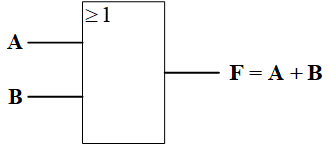
\includegraphics[width=0.32\linewidth]{Figure/或逻辑电路.png}
	\caption{或门逻辑符号}
	\label{fig:或门逻辑符号}
\end{figure}

或逻辑真值表如下：

\begin{table}[H]
\centering
\caption{或逻辑真值表}
\label{tab:真值表:或}
\begin{tabular}{cc|c}
	\toprule
	$A$ & $B$ & $F=A+B$ \\
	\midrule
	0 & 0 & 0 \\
	0 & 1 & 1 \\
	1 & 0 & 1 \\
	1 & 1 & 1 \\
	\bottomrule
\end{tabular}
\end{table}

\begin{note}
	与门和或门均可以有多个输入端。
\end{note}

\subsection{非逻辑运算}
\label{sec:非逻辑运算}

\begin{definition}[非逻辑运算]
	假定事件 $F$ 成立与否同条件 $A$ 的具备与否有关：若 $A$ 具备，则 $F$ 不成立；若 $A$ 不具备，则 $F$ 成立。$F$ 和 $A$ 之间的这种因果关系称为“非”逻辑关系，其函数式为 $F=\overline{A}$。
\end{definition}

非门逻辑符号如下：

\begin{figure}[H]
	\centering
	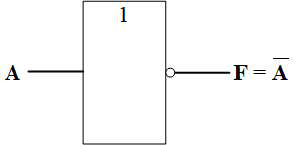
\includegraphics[width=0.3\linewidth]{Figure/非逻辑电路.png}
	\caption{非门逻辑符号}
	\label{fig:非门逻辑符号}
\end{figure}

非逻辑真值表如下：

\begin{table}[H]
\centering
\caption{非逻辑真值表}
\label{tab:真值表:非}
\begin{tabular}{c|c}
	\toprule
	$A$ & $F=\overline{A}$ \\
	\midrule
	0 & 1 \\
	1 & 0 \\
	\bottomrule
\end{tabular}
\end{table}

\section{复合逻辑运算}
\label{sec:复合逻辑运算}

\subsection{与非逻辑}
\label{sec:与非逻辑}

与非逻辑由与逻辑和非逻辑组合而成，函数式为 $F=\overline{A\cdot B}=\overline{AB}$。

\begin{figure}[H]
	\centering
	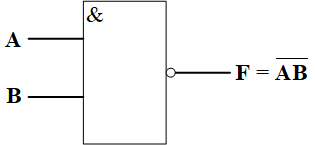
\includegraphics[width=0.3\linewidth]{Figure/与非逻辑电路.png}
	\caption{与非门逻辑符号}
	\label{fig:与非门逻辑符号}
\end{figure}

与非逻辑真值表如下：

\begin{table}[H]
\centering
\caption{与非逻辑真值表}
\label{tab:真值表:与非}
\begin{tabular}{cc|c}
	\toprule
	$A$ & $B$ & $F=\overline{AB}$ \\
	\midrule
	0 & 0 & 1 \\
	0 & 1 & 1 \\
	1 & 0 & 1 \\
	1 & 1 & 0 \\
	\bottomrule
\end{tabular}
\end{table}

\subsection{或非逻辑}
\label{sec:或非逻辑}

或非逻辑由或逻辑和非逻辑组合而成，函数式为 $F=\overline{A+B}$。

\begin{figure}[H]
	\centering
	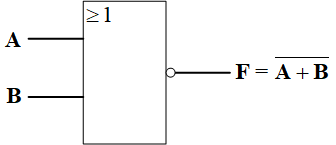
\includegraphics[width=0.32\linewidth]{Figure/或非逻辑电路.png}
	\caption{或非门逻辑符号}
	\label{fig:或非门逻辑符号}
\end{figure}

或非逻辑真值表如下：

\begin{table}[H]
\centering
\caption{或非逻辑真值表}
\label{tab:真值表:或非}
\begin{tabular}{cc|c}
	\toprule
	$A$ & $B$ & $F=\overline{A+B}$ \\
	\midrule
	0 & 0 & 1 \\
	0 & 1 & 0 \\
	1 & 0 & 0 \\
	1 & 1 & 0 \\
	\bottomrule
\end{tabular}
\end{table}

\subsection{与或非逻辑}
\label{sec:与或非逻辑}

与或非逻辑由与、或、非三种逻辑组合而成，函数式为 $F=\overline{AB+CD}$。

\begin{figure}[H]
	\centering
	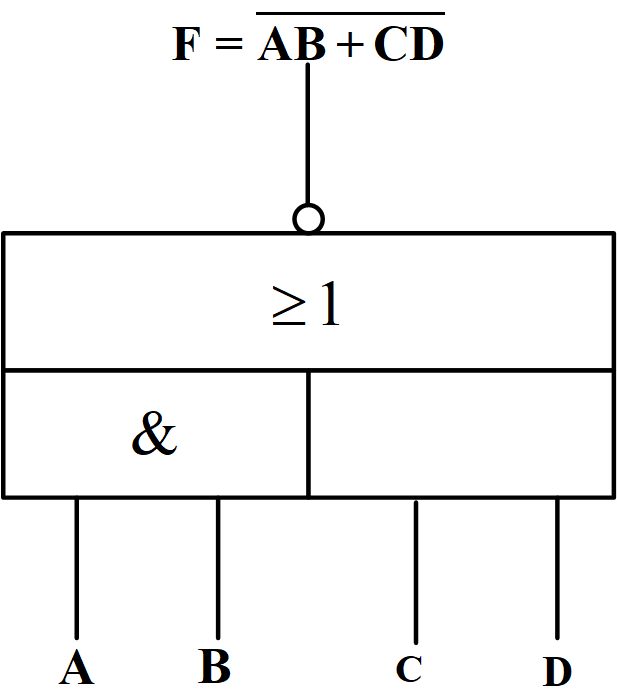
\includegraphics[width=0.42\linewidth]{Figure/与或非门逻辑符号.png}
	\caption{与或非门逻辑符号}
	\label{fig:与或非门逻辑符号}
\end{figure}

\subsection{异或逻辑}
\label{sec:异或逻辑}

异或逻辑的函数式为 $F=\overline{A}B+A\overline{B}=A\oplus B$，口诀：\textcolor{red}{相同得“0”，相异得“1”}。

\begin{figure}[H]
	\centering
	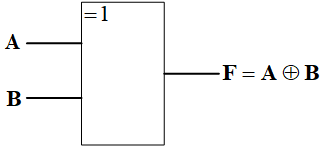
\includegraphics[width=0.32\linewidth]{Figure/异或逻辑电路.png}
	\caption{异或门逻辑符号}
	\label{fig:异或门逻辑符号}
\end{figure}

异或逻辑真值表如下：

\begin{table}[H]
\centering
\caption{异或逻辑真值表}
\label{tab:真值表:异或}
\begin{tabular}{cc|c}
	\toprule
	$A$ & $B$ & $F=A\oplus B$ \\
	\midrule
	0 & 0 & 0 \\
	0 & 1 & 1 \\
	1 & 0 & 1 \\
	1 & 1 & 0 \\
	\bottomrule
\end{tabular}
\end{table}

\subsection{同或逻辑}
\label{sec:同或逻辑}

同或逻辑的函数式为 $F=\overline{A}\,\overline{B}+AB=A\odot B$，口诀：\textcolor{red}{相同得“1”，相异得“0”}。

同或和异或互为反函数，即
\begin{equation}
	A\oplus B=\overline{A\odot B}
	\label{eq:复合:异或同或互为反}
\end{equation}

\begin{figure}[H]
	\centering
	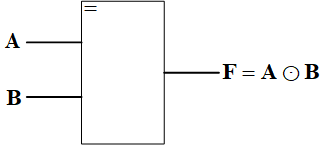
\includegraphics[width=0.32\linewidth]{Figure/同或逻辑电路.png}
	\caption{同或门逻辑符号}
	\label{fig:同或门逻辑符号}
\end{figure}

同或逻辑真值表如下：

\begin{table}[H]
\centering
\caption{同或逻辑真值表}
\label{tab:真值表:同或}
\begin{tabular}{cc|c}
	\toprule
	$A$ & $B$ & $F=A\odot B$ \\
	\midrule
	0 & 0 & 1 \\
	0 & 1 & 0 \\
	1 & 0 & 0 \\
	1 & 1 & 1 \\
	\bottomrule
\end{tabular}
\end{table}

\section{逻辑电平及正、负逻辑}
\label{sec:逻辑电平}

门电路的输入、输出为二值信号，用“0”和“1”表示，这里的“0”、“1”一般用两个不同电平值来表示。

\begin{definition}[正逻辑与负逻辑]
	\begin{itemize}
		\item \textbf{正逻辑}：若用高电平 $V_H$ 表示逻辑“1”，用低电平 $V_L$ 表示逻辑“0”，则称为正逻辑约定，简称正逻辑；
		\item \textbf{负逻辑}：若用高电平 $V_H$ 表示逻辑“0”，用低电平 $V_L$ 表示逻辑“1”，则称为负逻辑约定，简称负逻辑。
	\end{itemize}
	一般采取正逻辑表示。
\end{definition}

\begin{note}
	对一个特定的逻辑门，采用不同的逻辑表示时，其门的名称也就不同。
\end{note}

\section{基本定律和规则}
\label{sec:基本定律和规则}

\subsection{逻辑函数的相等}
\label{sec:逻辑函数的相等}

设有两个逻辑函数
\begin{equation}
	F_1=f_1(A_1,A_2,\cdots,A_n),\qquad
	F_2=f_2(A_1,A_2,\cdots,A_n)
	\label{eq:定律:函数定义}
\end{equation}
如果对于 $A_1,A_2,\cdots,A_n$ 的任何一组取值（共 $2^n$ 组），$F_1$ 和 $F_2$ 均相等，则称 $F_1$ 和 $F_2$ 相等。

因此，如两个函数的真值表相等，则这两个函数一定相等。

\subsection{基本定律}
\label{sec:基本定律}

\begin{table}[H]
\centering
\caption{逻辑代数的基本定律}
\label{tab:定律:基本定律}
\begin{tabular}{lcc}
	\toprule
	定律 & 与形式 & 或形式 \\
	\midrule
	① 0-1 律 & $A\cdot0=0$ & $A+1=1$ \\
	② 自等律 & $A\cdot1=A$ & $A+0=A$ \\
	③ 重叠律 & $A\cdot A=A$ & $A+A=A$ \\
	④ 互补律 & $A\cdot\overline{A}=0$ & $A+\overline{A}=1$ \\
	⑤ 交换律 & $A\cdot B=B\cdot A$ & $A+B=B+A$ \\
	⑥ 结合律 & $A(BC)=(AB)C$ & $A+(B+C)=(A+B)+C$ \\
	⑦ 分配律 & $A(B+C)=AB+AC$ & $A+BC=(A+B)(A+C)$ \\
	⑧ 反演律 & $\overline{A+B}=\overline{A}\cdot\overline{B}$ & $\overline{AB}=\overline{A}+\overline{B}$ \\
	\bottomrule
\end{tabular}
\end{table}

反演律也称\textbf{德·摩根定理}，是一个非常有用的定理。

\subsection{逻辑代数的三条规则}
\label{sec:逻辑代数的三条规则}

\subsubsection{代入规则}
\label{sec:代入规则}

任何一个含有变量 $x$ 的等式，如果将所有出现 $x$ 的位置，都用一个逻辑函数式 $F$ 代替，则等式仍然成立。

\subsubsection{反演规则}
\label{sec:反演规则}

设 $F$ 为任意逻辑表达式，若将 $F$ 中所有运算符、常量及变量作如下变换：

\begin{figure}[H]
	\centering
	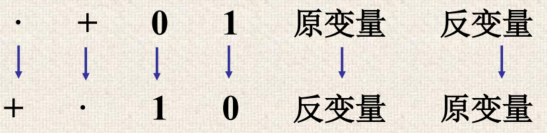
\includegraphics[width=0.75\linewidth]{Figure/反函数定义.png}
	\caption{反函数的变换规则}
	\label{fig:反函数定义}
\end{figure}

则所得新的逻辑式即为 $F$ 的反函数，记为 $\overline{F}$。

\textbf{注意}：
\begin{enumerate}
	\item 保持原式运算的优先次序；
	\item 原式中的不属于单变量上的非号不变。
\end{enumerate}

\subsubsection{对偶规则}
\label{sec:对偶规则}

设 $F$ 为任意逻辑表达式，若将 $F$ 中所有运算符和常量作如下变换：

\begin{figure}[H]
	\centering
	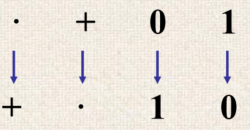
\includegraphics[width=0.4\linewidth]{Figure/对偶式定义.png}
	\caption{对偶式的变换规则}
	\label{fig:对偶式定义}
\end{figure}

则所得新的逻辑表达式即为 $F$ 的对偶式，记为 $F'$。
